\vspace{-0.6cm}

\section*{Appendix}

{\color{blue}
\section{Parameter settings}

\subsection*{Setting for $\alpha,\beta$-Crown}

The networks were already tested by $\alpha,\beta$-Crown \cite{crown}. We thus simply reused the parameter files from \href{https://github.com/Verified-Intelligence/alpha-beta-CROWN/blob/main/complete_verifier/exp_configs/beta_crown/}{their Github}, 
except for time-out which we explicitly mention.

e.g., for CNN-B-Adv: "solver: batch size: 512 beta-crown: iteration: 20" and
for MNIST 5x100: "solver: batch size: 1024 beta-crown: iteration: 20".

We did not experiment with cutting planes (GCP-CROWN \cite{cutting}), as it needs an additional package, namely IBM CPLEX solver, we do not have access to. From \cite{cutting}, the number of undecided inputs of GCP-CROWN is $\leq 2\%$ better than $\alpha,\beta$-Crown on the DNNs we experimented with, far from the $10-40\%$ improvement seen from Hybrid MILP. The conclusion are thus unchanged.
}

\subsection*{Setting for Hybrid MILP}


Hybird MILP first call $\alpha,\beta$-Crown with short time-out (TO), then call partial MILP on those inputs which was neither certified nor falsified by this run of $\alpha,\beta$-Crown. We are using two settings of TO, for smaller DNNs we use T0$=10s$, and for the two larger ones, we use TO$=30s$.

The setting for partial MILP for fully-connected DNNs is about how many neurons need to be opened (once set, the selection is automatic). The runtime depending crucially upon the number of open ReLU neurons, we set it quite tightly, only allowing few neuron deviation to accommodate to a particularly accurate/inaccurate bound computation (measure by the weight of the remaining Utility function). As complexity increases with the layer considered, as the size of the MILP model grows, we lower this number with the depth, only committing to an intermediate number for the output neuron (the number of output neurons  is smaller than hidden layer, and this is the most important computation). We experimentally set this number so that each computing the bounds in each hidden layer takes around the same time. Remember that in layer 1, partial MILP is not necessary and propagating bounds using interval arithmetic is already exact. We open [48,48] to compute bounds for hidden layer 2, [21,24] for layer 3, [11,14] for layer 4, [6,9] for layer 5, [3,6] for layer 6, [2,5] for layer 7, [1,4] for hidden layer 8 (if any), and we open [14,17] for the output layer.
{\color{blue} The exact number of open nodes in the range [a,a+3] is decided automatically for each neuron being computed : ReLUs are ranked according to their value by Utility, and the a top ReLUs are open. Then, ReLUs ranked a+1,a+2, a+3 are opened if their Utility value is larger than a small threshold. We set the threshold at 0.01. It should be seen as a way to save runtime when Utility knows that the next node by ranking (a+i) will not impact accuracy much (thanks to the upper bound from Proposition \ref{prop2}).}

\begin{table}[b!]
	\centering
	\begin{tabular}{||l||c|c||}
		\hline \hline
		Network & TO for $\alpha,\beta$-Crown  & Minimum number of Open neurons  \\ 		  
		\hline
		MNIST $5 \times 100$ & 10s  & 48,21,11,6,14  \\ \hline
		MNIST $5 \times 200$ & 10s & 48,21,11,6,14  \\ \hline
		MNIST $8 \times 100$ & 10s  & 48,21,11,6,3,2,1,14  \\ \hline
		MNIST $8 \times 200$ & 10s & 48,21,11,6,3,2,1,14  \\ \hline
		MNIST $6 \times 500$ & 30s & 48,21,11,6,3,14 \\ \hline
		CIFAR CNN-B-adv & 30s & 200, 0, 45 \\ \hline \hline
	\end{tabular}
	\caption{Settings of Hybrid MILP for the different {\em hard} instances}
	\label{table20}
	\end{table}


For convolutional CNNs, the strategy is adapted, as there is much more neurons, but in a shallower architecture and not fully connected. 
The second layer is computed accurately, opening 200 neurons, which is manageable as there is only one ReLU layer to consider, and accuracy here is crucial.
We do not open any nodes in the third layer (the first fully connected layer) if the output layer is the next one (which is the case for CNN-B-Adv), and instead rely on the choice of important nodes for the output layer. Otherwise, we open 20 neurons.
In the output layer, we open at least 45 neurons (there is less output neurons than nodes in the previous layer), and enlarge the number of open neurons (up to 300) till we find an upper bound, that is a best current MILP solution, of around +0.1 (this 0.1 was experimentally set as target, a good balance between accuracy and efficiency), and compute a guaranteed lower bound (the goal is to guarantee the bound is $>0$).

In Table \ref{table20}, we sum-up the TO and minimum open numbers for each DNN considered.

{\color{blue}
$\alpha,\beta$-Crown uses massively parallel ($>$4096 threads) GPU, while Partial MILP uses 20 CPU-threads.}

Notice that a different balance between accuracy and runtime could be set. For instance, we set up the numbers of open neurons to have similar runtime as Refined $\beta$-Crown for the first 4 DNNs ($50s-100s$). We could easily target better accuracy (e.g. for $8 \times 100$ with a relatively high $15\%$ undecided images) by increasing the number of open neurons, with a trade-off on runtime (current runtime is at $61s$).
By comparison, the sweet spot for $\alpha,\beta$-Crown seems to be around TO$=30s$, enlarging the time-out having very little impact on accuracy but large impact on runtime
(Table \ref{table_beta}).


{\color{blue}
Last, for Gurobi, we use a custom MIP-Gap (from $0.001$ to $0.1$) and time-out parameters, depending on the seen improvement and the possibility to make a node stable. This is low level implementation details that will be available in the code once the paper is accepted.
}





{\color{blue}

\section{Pseudocode and Complexity Analysis}	

\SetKwInput{KwInput}{Input}
\SetKwInput{KwOutput}{Output}

\begin{algorithm}[h!]
	\caption{pMILP($K$)}
	\label{algo1}
	\KwInput{Bounds $[\alpha_n,\beta_n]$ for input nodes $n$ at layer $0$ (input neighbourhood)}
	
	\KwOutput{Bounds $[\alpha_n,\beta_n]$ for every node $n$}
	
	\For{layer $k=1 \cdots \ell$}{
		\For{neuron $n$ in layer $k$}{
			
			Compute $X$ a set of $K$ nodes with the highest Utility for target neuron $n$.
			
			Run MILP$_X$ to obtain $[\alpha_n,\beta_n]$ from bounds of neurons in layers $< k$
		}
	}
\end{algorithm}	

%We then analyse its complexity.
%First, notice that the complexity to rnu Utility is negligible wrt the Run MILP$_X$.

We provide the pseudo code for pMILP in Algorithm \ref{algo1}.
pMILP($K$) has a worst case complexity bounded by $O(N \cdot \MILP(N,K))$, 
where $N$ is the number of nodes of the DNN, and $\MILP(N,K)$ is the complexity of solving a MILP program with $K$ integer variables and $N$ linear variables.
We have $\MILP(N,K) \leq 2^K \LP(N)$ where $\LP(N)$ is the Polynomial time to solve a Linear Program with $N$ variables, $2^K$ being an upper bound. Solvers like Gurobi are quite adept and usually do not need to evaluate all $2^K$ ReLU configurations to deduce the bounds.
It is worth mentioning that the "for" loop iterating over neurons $n$ in layer $k$ (line 2) can be executed in parallel, because the computation only depends on bounds from preceding layers, not the current layer $k$. 
%This parallelization results in a time complexity of $O(\sum_{i=1}^{\ell} \MILP(N_{i-1},K))$, where $\ell$ denotes the total number of layers and $N_i$ the count of neurons in layers $0, ..., i$. 
%pMILP uses 20 threads.


If $K$ is sufficiently small, 
%Algorithm \ref{algo1} invokes many MILP (e.g., using Gurobi) with a manageable number of %integer variables. 
this approach is expected to be efficient. 
The crucial part is thus to find few neurons which are particularly important when computing neuron $n$. This is where our novel Utility function outperforms previous solutions, by using an call to an (LP) solver to obtain a solution, which is novel as far as we know. This solutions allows to optimizing the choice of open nodes for the particular input considers, and appears significantly better than previous attempts, explaining the efficiency of the method.

For comparison, refined $\beta$-Crown and refined Prima used all the nodes up to a certain layer as binary variables, which is particularly inefficient, see Table \ref{table12} and Fig. \ref{fig4}. Hence, it can only be applied to small DNNs (it is implemented only up to MNNIST 8x200), while pMILP scales to at least 20.000 neurons (CNN-B-Adv).
\cite{DivideAndSlide} is the closest to pMILP, also implementing a choice of nodes as binary variables. However, their choice is particularly inefficient, as revealed by Table  
\ref{tab:example1}, needing 4 times the number of open nodes for the same accuracy as our Utility function.




\section{Ablation studies}	

In this section, we consider ablation studies to understand how each feature enables the efficiency of pMILP.

\subsection*{Time scaling with open nodes}	

First, we explore the time scaling with different number of open nodes, for our full Utility function using nodes in the last two layers (Layer 1 and 2), providing finer details than in Table 3, with the same setting, i.e. previous layer being computed with full MILP.





\begin{table}[h!]
		\centering
		\hspace*{4ex}
		\begin{subtable}[b]{0.45\textwidth}
		\begin{tabular}{|c|c|c|}
		\hline
		$|X|$ & Time & Uncertainty\\ 
		\hline	0 & 2.6 & 1.760946128\\
		\hline	1 & 7.3 & 1.702986873\\
		\hline	2 & 11.1 & 1.65469034\\
		\hline	3 & 16.3 & 1.612137282\\
		\hline	4 & 15.5 & 1.571001109\\
		\hline	5 & 15.7 & 1.531925404\\
		\hline	6 & 15.8 & 1.49535638\\
		\hline	7 & 16.4 & 1.46189314\\
		\hline	8 &  15.8 & 1.4299535\\
		\hline	9 &  17.2 & 1.4006364\\
		\hline	10 & 22.5 & 1.3711203\\
		\hline	11 & 27.2 & 1.3438245\\
		\hline	12 & 21.6 & 1.3183356\\
		\hline	13 & 28.7 & 1.2938690\\
		\hline	14 & 29.6 & 1.2690507\\
		\hline	15 & 24.5 & 1.2475106\\
		\hline
	  \end{tabular}
	\end{subtable}
	\hfill
	\begin{subtable}[b]{0.45\textwidth}
		\begin{tabular}{|c|c|c|}
			\hline
			$|X|$ & Time & Uncertainty\\ 
		\hline	16 & 31.9 & 1.2243065\\
		\hline	17 & 28.6 & 1.2031791\\
		\hline	18 & 30.4 & 1.1839474\\
		\hline	19 & 34.0 & 1.1644653\\
		\hline	20 & 42.1 & 1.1456181\\
		\hline	21 & 47.6 & 1.1261252\\
		\hline	22 & 62.7 & 1.1089745\\
		\hline	23 & 70.0 & 1.0931242\\
		\hline	24 & 70.8 & 1.0773088\\
		\hline	25 & 139.9 & 1.060928\\
		\hline	26 & 154.2 & 1.045715\\
		\hline	27 & 213.1 & 1.030605 \\
		\hline	28 & 211.3 & 1.016058\\
		\hline	29 & 373.1 & 1.001374\\
		\hline max=116 & 3300 & 0.895\\ 
		\hline		
	  \end{tabular}
     \end{subtable}
	  \caption{Time and uncertainty scaling of pMILP with number of nodes.}
    	\label{table14}
\end{table}


\begin{figure}[b!]
	\hspace*{-0.8cm}
	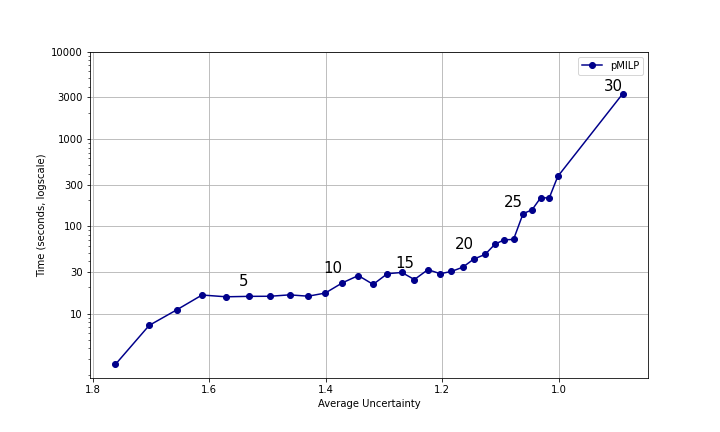
\includegraphics[scale=0.6]{Layer3_comparison}.
	\caption{Time and uncertainty scaling of pMILP with number of nodes.
	Time is using logscale.}
	\label{fig3}
\end{figure}


The exponential complexity with the number of nodes can be seen on Figure \ref{fig3}, where time is represented using logarithmic scale. The flat area in the middle is Gurobi having good heuristic to avoid considering all $2^K$ cases when $K<21$ is not too large, but not working so well for $K>25$. Notice that when certifying, pMILP uses $|X| \in$ 21-24, which is a good trade off between time and accuracy.


We also provide in Table \ref{tab:example1} the raw numbers used to produce Figure \ref{fig_table3}.
Further, we tested with the SR and FSB heuristics \cite{BaB}, that chooses nodes to branch on for BaB (Branch and Bound). When used instead to open nodes for pMILP, SR and FSB result in particularly low accuracy:
even though SR, FSB and \cite{DivideAndSlide} heuristic are all choosing ReLUs based on sensitivity of the target neuron $z$, SR and FSB are worse than \cite{DivideAndSlide} which only opens neurons one layer before (except when all ReLUs of the previous layers are open), and far worse than Utility. Further, FSB is performing worse than SR when choosing nodes for pMILP, while to choose nodes to branch on for BaB, it is the opposite. This likely means that the heuristic to choose nodes to branch for BaB is not adapted to choose nodes to open for pMILP.

\begin{table}[h!]	
	\centering
	\begin{tabular}{|c||c|c|c|c|c||c|c|c|c|}
		\hline
			&\multicolumn{5}{c||}{$X \subseteq$ Layer 2, max $=55$}&\multicolumn{4}{c|}{$X \subseteq$ Layers 1\&2, max $=116$} \\\cline{2-10}
		\text{$|X|$}  & \text{Random} & Huang &SR&FSB& \bf Utility& \text{Random} & SR & FSB &\bf Utility\\ \hline
		\hline
		0  (LP) &   1.761  &1.761&1.761&1.761& 1.761 & 1.761  &  1.761& 1.761 & 1.761\\ \hline \hline
		5  &   1.729&1.704 &1.7200&1.7197& 1.603&  1.729& 1.7133 & 1.7149 & \bf 1.532 \\ \hline
		10  &  1.701 &  1.651 &1.6840&1.6851&1.517& 1.696 & 1.6674& 1.6714 & \bf  1.371\\ \hline
		15  & 1.671 &  1.599 &1.6502& 1.6516&1.466&  1.653& 1.6230& 1.6251 & \bf  1.247\\ \hline
		20  &  1.635 & 1.557&1.6190&1.6199&1.438 & 1.619 &1.5764 & 1.5812 & \bf  1.145\\ \hline
		25  &  1.601 & 1.519 &1.5887&1.5886&1.427&  1.586 &1.5322 & 1.5388 & \bf 1.061\\ \hline
		30  & 1.574 & 1.489 &1.5584&1.5604&1.425& 1.546 &  1.4914& 1.4982 & \bf  0.989 \\ \hline
		35  &  1.542 & 1.465&1.5289&1.5305&1.424 & 1.502 & 1.4481 & 1.4600 & \bf 0.934 \\ \hline
		40  & 1.512 & 1.447 &1.4985&1.5001&1.424& 1.469 & 1.4070& 1.4187 & \bf 0.921 \\ \hline \hline
		max & 1.424  &1.424&1.424&1.424& 1.424 & 0.895 & 0.895 & 0.895 & 0.895   \\ \hline
	\end{tabular}
	\caption{Average uncertainty of $\MILP_X$ for nodes of the third layer, for $X$ with $K$ ReLU nodes of the (1st and) 2nd layer, chosen by our {\bf Utility} function vs \cite{ DivideAndSlide} vs SR vs FSB vs random choice.}
	\label{tab:example1}
	%\vspace{-0.6cm}
\end{table}



	\begin{figure}[h!]
		\centering
		\vspace*{-0.3cm}
		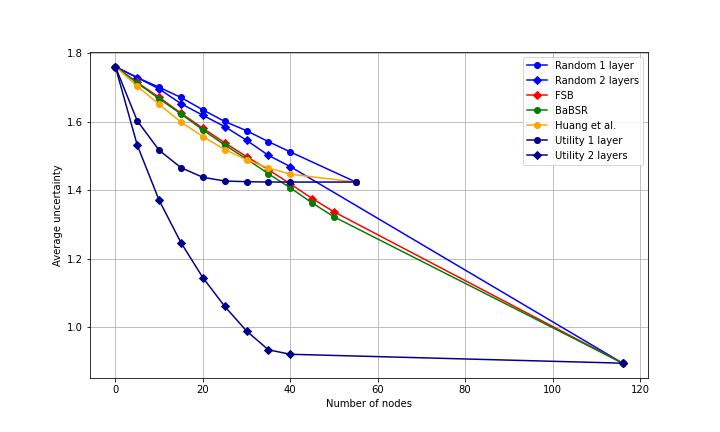
\includegraphics[height=9cm]{New Plot for table 3}.
		\vspace*{-0.4cm}
		\caption{Average uncertainty of $\MILP_X$ for nodes of the third layer, with ReLU nodes of the (1st and) 2nd layer, chosen by our {\bf Utility} function vs \cite{DivideAndSlide} vs vs SR vs FSB vs random.}
		\label{fig_table3_new}
	\end{figure}




\newpage

\subsubsection*{Usefulness of computing previous layers accurately}	


Then, we explore the usefulness of computing accurately each layer inductively.
For that, we keep the setting of Figure \ref{fig3} / Table \ref{table14}, but computing the previous layer with LP rather than with full MILP.


\begin{figure}[h!]
	\hspace*{-0.8cm}
	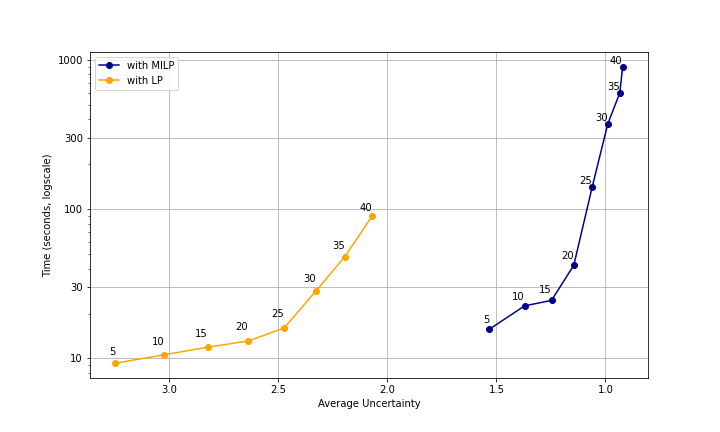
\includegraphics[scale=0.6]{Layer3_comparison_LP}.
	\caption{Comparison of accuracy in layer 3 when layer 2 is computed inaccurately using LP vs when layer 2 computed accurately using MILP.
	Time is using logscale.}
	\label{fig3LP}
\end{figure}








\begin{table}[h!]
	\centering
\begin{tabular}{|c|c|c|c|}
	\hline
	$|X|$ & Time &  With LP for layer 2 & With MILP for layer 2 \\ 
	\hline	5 & 9.3 & 3.24737  &1.532\\
	\hline	10 & 10.6 & 3.02214 & 1.371\\
	\hline	15 & 11.9 & 2.82383  &1.247\\
	\hline	20 & 13.1 & 2.63862 & 1.145\\
	\hline	25 & 16.0 & 2.47324 & 1.061\\
	\hline	30 & 28.3 & 2.32793  &0.989\\
	\hline	35 & 48.1 & 2.19506 & 0.934\\
	\hline	40 & 89.4 & 2.07107 & 0.921\\	
	\hline	
\end{tabular}
\caption{Comparison of accuracy in layer 3 when layer 2 is computed inaccurately using LP vs when layer 2 computed accurately using MILP.}
\label{table15}
\end{table}



This experiment explains the rationale to use divide and conquer protocol, using many calls
(one for each neuron) with relatively small number $|X|$ of open nodes rather than fewer calls to MILP with larger number $|X|$ of open nodes. This is clear already with only 1 layer before.


	
%		\begin{figure}[h]\hspace*{-1cm}
%		\includegraphics[scale=0.6]{Layzr3_comparison.png}.
%		\caption{Comparison of layer3 when layer 1 is MILP or LP}
%\label{fig4}
%	\end{figure}


\newpage

\subsubsection*{restricting number of open nodes (pMILP) vs setting time-outs (full MILP)}	

Running full MILP till a small MIP-Gap (typically 0.001) is reached is extremely time inefficient.

Instead, the standard strategy is to set a reasonable time-out and use whatever bound has been generated. We compare this standard strategy with the pMILP strategy of setting a priori a number of open nodes.

\begin{figure}[h!]\hspace*{-0.8cm}
	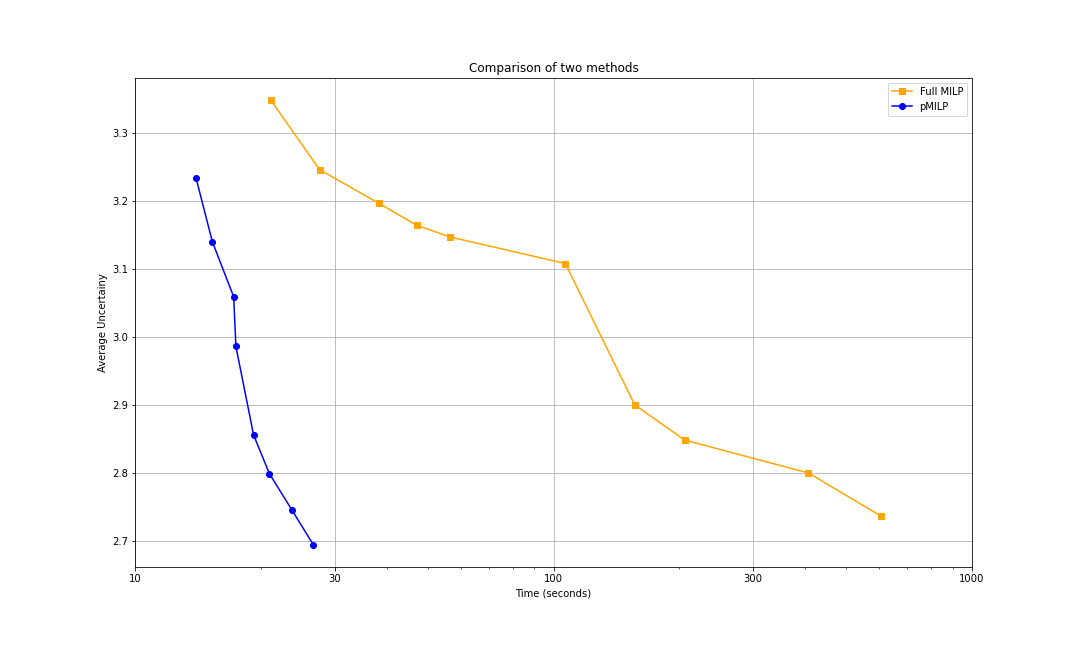
\includegraphics[scale=0.6]{Layer7_comparison.png}.
	\caption{Comparison of uncertainty at layer 7 for full MILP with different time-outs vs pMILP with different number of open nodes. Time is using logscale.}
	\label{fig4}
\end{figure}



\begin{table}[h!]
	\centering
	\hspace*{4ex}
\begin{subtable}[b]{0.45\textwidth}
	\centering
		\begin{tabular}{|c|c|c|}
	\hline
		$|X|$ & Time & Uncertainty\\ 
	\hline1 &	14 & 3.233021901\\
\hline	2 & 15.2 & 3.140309921\\
\hline	3 & 17.21 & 3.059083103\\
\hline 4 &	17.4 & 2.986166762\\
\hline	5 &19.2 & 2.856229765\\
\hline	6 &20.9 & 2.799248232\\
\hline	7 &23.7 & 2.746167245\\
\hline	8 &26.6 & 2.69485246\\	
	\hline
	\end{tabular}
	\caption{pMILP}
\end{subtable}
\hfill
\begin{subtable}[b]{0.45\textwidth}
	\centering
		\begin{tabular}{|c|c|}
		\hline
		Time & Uncertainty\\ 
		\hline	21.1 & 3.348236261\\
		\hline	27.6 & 3.24604282\\
		\hline	38.2 & 3.196640184\\
		\hline	47.1 & 3.164298172\\
		\hline	56.7 & 3.146913614\\
		\hline	106.7 & 3.108035223\\
		\hline	156.3 & 2.900438725\\
		\hline	205.8 & 2.848648426\\	
		\hline	406.7 & 2.800268264 \\	
		\hline	606.1 & 2.737064255\\	
		\hline
	\end{tabular}
		\caption{full MILP}
\end{subtable}
	\caption{Comparison of bounding the number of nodes for pMILP and 
	using different time outs for full MILP. In both settings, lower and upper bounds of previous layers are the same (computed by pMILP).}
	\label{table12}
	\end{table}

	

	

pMILP obtains 2.8 accuracy in $<21$ seconds (with 7 open nodes), while full MILP needs 400 seconds to obtain it, a 19x speed up. For 2.7 accuracy, the speedup is $>>$ 22.



Figure \ref{fig4} shows that choosing nodes is much more efficient for time/accuracy trade-off than setting time outs and use full MILP. And this is for the smallest DNN we considered (500 hidden neurons, far from the biggest 20k neuron DNN we experimented with)


\section{Comparison with other DNN verifiers}

In the following, we provide results comparing $\alpha,\beta$-Crown to other verifiers, to justify our use of $\alpha,\beta$-Crown as state of the art for efficient verifiers as main source of comparison to Hybrid MILP for hard DNN instance.


\subsection*{Comparison $\alpha,\beta$-Crown vs PRIMA}


\begin{table}[b!]
	\centering
	\begin{tabular}{||l||c|c||c||}
		\hline \hline
		Network & $\alpha,\beta$-Crown & Refined $\beta$-Crown & PRIMA \\ 		  
		\hline
		MNIST $5 \times 100$ & N/A  & 14.3\% (102s) & 33.2\% (159s)\\ \hline
		MNIST $5 \times 200$ & N/A & 13.7\% (86s) & 21.1\% (224s) \\ \hline
		MNIST $8 \times 100$ & N/A  & 20.0\% (103s) & 39.2\% (301s)   \\ \hline
		MNIST $8 \times 200$ & N/A & 17.6\% (95s) & 28.7\% (395s)  \\ \hline
		MNIST $6 \times 500$ & 51\% (16s) & $-$ & 64\% (117s) \\ \hline
		CIFAR CNN-B-adv & 18.5\% (32s) & $-$ & 27\% (344s)\\ \hline \hline
		CIFAR ResNet & 0\% (2s) & $-$ & 0\% (2s) \\ \hline \hline
	\end{tabular}
	\caption{Undecided images ($\%$, {\em lower is better}), as computed by $\alpha,\beta$-Crown, Refined $\beta$-Crown, and PRIMA, as reported in \cite{crown}, except for $6 \times 500$ that we run ourselves. N/A means that \cite{crown} did not report the numbers, while $-$ means that Refined $\beta$-Crown cannot be run on these DNNs.}
	\label{table9}
	%\begin{tablenotes}
	%	\footnotesize
%		\item Most data is directly from \cite{crown}. N/A means no data either in \cite{crown} or by our running.
%		\item  $^*$ The data in this row is from our own running on first 100 images of the MNIST dataset.
%		\item  $^{**}$ The data is from \cite{crown} on first 200 images of the CIFAR10 dataset.
%	\end{tablenotes}
	\end{table}


	PRIMA \cite{prima} is a major verifier in the ERAN toolkit. In Table \ref{table9}, we report the comparison between PRIMA and $\alpha,\beta$-Crown, mainly from \cite{crown}. The setting is mainly similar from ours, but numbers are not perfectly comparable as the images tested are not  exactly the same (1000 first or 200 first images for CNN-B-Adv), vs 100 first in Tables \ref{table_hybrid}, \ref{table_beta}. Also, time-out settings and hardware are slightly different. The overall picture is anyway the same.


Analysis: On the 4 smallest MNIST networks, PRIMA uses a refined path comparable with Refined $\beta$-Crown. However, it is slower and less accurate than Refined $\beta$-Crown.
On larger {\em hard} networks, PRIMA has also more undecided images than $\alpha,\beta$-Crown, while the runtime is $>5$ times larger.
Hence, Hybrid MILP is more accurate than Prima with similar runtime or faster.

Notice that kPoly \cite{kpoly}, OptC2V \cite{optC2V}, SDP-FO \cite{SDPFI} numbers were also reported in \cite{crown} on these networks, with even more unfavorable results.

\subsection*{Comparison $\alpha,\beta$-Crown vs MN-BaB}

MN-BaB \cite{ferrari2022complete} is an improvement built over PRIMA, using a similar Branch and Bound technique as used in $\alpha,\beta$-Crown. Results in \cite{ferrari2022complete}
are close to those of $\alpha,\beta$-Crown. However, none of the {\em hard} networks from \cite{crown} that we consider have been tested. We thus tested three representative {\em hard} DNNs (first 100 images) to understand how MN-BaB fairs on such hard instances, and report the numbers in Table \ref{table10}. Results are directly comparable with Table \ref{table_hybrid}.


\begin{table}[h!]
	\centering
	\begin{tabular}{||l||c|c||c|c||}
		\hline \hline
		 & $\alpha,\beta$-Crown & $\alpha,\beta$-Crown & MN-BaB & MN-BaB \\ 
		 Network & TO=30s & TO=2000s &  TO=30s & TO=2000s \\ 
		\hline
		MNIST $5 \times 100$ & 55\% (19s) & 50\%(1026s) & 60\% (19s) & 50\% (1027s) \\ \hline
		MNIST $6 \times 500$ & 51\% (16s) & 50\% (1002s) & 58\% (18s) & 55\% (1036s) \\ \hline
		CIFAR CNN-B-adv & 22\% (8.7s) & 20\% (373s) & 43\% (14s) & 24\% (576s) \\ \hline 
	\end{tabular}
	\caption{Undecided images ($\%$, {\em lower is better}), as computed by $\alpha,\beta$-Crown, and MN-BaB}
	\label{table10}
\end{table}

Analysis: results reveal that MN-BaB is slightly slower and slightly less accurate than $\alpha,\beta$-Crown. Notice the specially high number of undecided images for CNN-B-Adv with TO=30s, probably meaning that 30s is too small for MN-BaB on this large DNN.
Hence, Hybrid MILP is more accurate than MN-BaB with similar runtime or faster.



	\subsection*{Comparison $\alpha,\beta$-Crown vs NNenum}

NNenum \cite{nnenum} is a complete verifier with good performance according to VNNcomp.
It was the only complete verifier tested in Table \ref{table_complete} to verify more images than $\alpha,\beta$-Crown. The experiments section in \cite{nnenum} does not report
the {\em hard} DNNs we are considering. We tried to experiment it on the same MNIST 
$6 \times 500$ and CIFAR CNN-B-adv as we did in Table \ref{table10} for MN-BaB. Unfortunately, on $6 \times 500$, buffer overflow were reported.
We report in Table \ref{table11} experiments with the same 2000s Time-out (it was $10 000s$ in Table \ref{table_complete})  for a fair comparison with $\alpha,\beta$-Crown, on both 
MNIST $5 \times 100$ and CIFAR CNN-B-Adv. 
On MNIST $5 \times 100$, NNenum is slightly more accurate than $\alpha,\beta$-Crown, but far from the accuracy Hybrid MILP.
On CIFAR CNN-B-adv, NNenum was much less accurate than $\alpha,\beta$-CROWN, and thus of Hybrid MILP. In both test, the runtime of NNenum was also much longer than for Hybrid MILP.


\begin{table}[h!]
	\centering
	\begin{tabular}{||l||c||c||c||c||}
		\hline \hline
		 & $\alpha,\beta$-Crown & NNenum & Hybrid\\ 
		 Network & TO=2000s &  TO=2000s & MILP\\ 
		\hline
		MNIST $5 \times 100$ & 50\%(1026s) & 44\% (1046s) & \bf 13\% (46s)\\ \hline
		CIFAR CNN-B-adv & 20\% (373s) & 40\% (1020s) & \bf 11\% (417s)\\ \hline 
	\end{tabular}
	\caption{Undecided images ($\%$, {\em lower is better}), as computed by $\alpha,\beta$-Crown and NNenum with 2000s time-out, and Hybrid MILP}.
	\label{table11}
\end{table}


{\color{blue}

\section{Average vs max time per pMILP call}

We provide in Table \ref{table112} the average as well as maximum time to perform $MILP_X$ calls as called by pMILP, on a given input: image 3 for MNIST, and image 76 for CIFAR10. 
For 6x500, we provide results for two different $\varepsilon$, following our test from Figure \ref{fig2}.

\begin{table}[h!]
	\centering
	\begin{tabular}{||l|c|c||}
		\hline
		Network & average time & maximum time \\ \hline
		MNIST 5$\times$100 & 0.41s & 1.87 \\
		$\epsilon = 0.026$ &  & \\  \hline
		MNIST 5$\times$200 &  0.75s & 5.31s \\ 
		$\epsilon = 0.015$ & & \\  \hline
		MNIST 8$\times$100 & 0.39s & 1.41s \\
		$\epsilon = 0.026$ & &  \\  \hline
		MNIST 8$\times$200 & 0.49s & 1.63s \\ 
		$\epsilon = 0.015$ & & \\  \hline
		MNIST 6$\times$500 & &   \\ 
		$\epsilon = 0.035$ & 1.4s & 3.5s \\ 
		$\epsilon = 0.1$ & 44.6s & 310s \\  \hline 
		CIFAR CNN-B-adv &  & \\
		$\epsilon = 2/255$& 1s & 609s \\ \hline \hline
	\end{tabular}
	\caption{average and maximum time per $\MILP_X$ calls for image 3 (MNIST) and image 76 (CIFAR10).}
	\label{table112}
\end{table}

Notice that DNN 6$\times$ 500 and $\epsilon=0.1$ is a very hard instance as being very close to the falsification $\epsilon \approx 0.11$. This is thus not representative of the average case. Also,  on this image 3, pMILP succeeds to verify $\epsilon= 1.054$, while $\alpha,\beta$-CROWN can only certify $\epsilon = 0.0467$ within the 10 000s Time-out.

For CNN-B-Adv, the very long maximum time for a MILP call is an outlier: it happens only for one output layer, for which the number $K$ of open nodes is particularly large (around 200 out of 20000 neurons) to certify this hard image 76. Indeed, the average time is at $1s$. Notice that this does not lead to a runtime of 20.000s, as 20 threads are used by pMILP 
in parallel (similar to competing solutions, except $\alpha,\beta$-CROWN which uses $>4096$ GPU cores).


}









\end{document}


\section{SR Heuristic for choosing nodes}

Here we provide the formula of BaB-SR from paper \cite{BaB}.

\begin{align*}
	\nu_{n+1} &= -1&\\
	\hat{\nu}_k &= W^T_kv_{k+1}, k = n,\cdots,1 &\\
	\nu_{k,j} &= \begin{cases}
		0  &\text{ if }u_{k[j]}<0 \hspace*{2ex}(j\in\mathcal{I}^-_k)\\
		\hat{\nu}_{k[j]} &\text{ if }l_{k[j]}>0 \hspace*{2.5ex}(j\in\mathcal{I}^-_k)\\
		\frac{u_{k[j]}}{u_{k[j]}-l_{k[j]}}[\hat{\nu}_{k[j]}]_+-\frac{u_{k[j]}}{u_{k[j]}-l_{k[j]}}[\hat{\nu}_{k[j]}]_-  &\text{ otherwise } \hspace*{3ex}(j\in\mathcal{I}_k)\\ 
	\end{cases}\\
	&\hspace*{22ex}\text{for } k = n,\cdots,2&
\end{align*}and\begin{align*}
	s_{i[j]} = |\max(v_{i[j]}b_{i-1[j]},(v_{i[j]}-1)b_{i-1[j]})-\frac{u_{k[j]}}{u_{k[j]}-l_{k[j]}}[\hat{\nu}_{k[j]}]_+|
\end{align*}


\begin{figure}[b!]
	\hspace*{-0.8cm}
	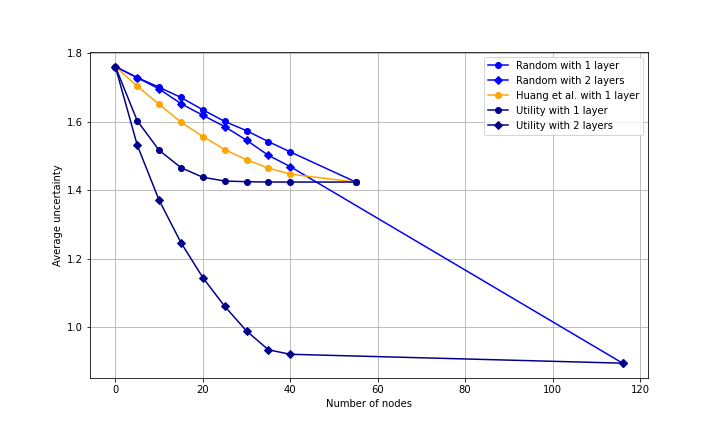
\includegraphics[scale=0.6]{Plot for table 3}.
	\caption{Plot for table 3}
	\label{fig_table3}
\end{figure}


\begin{table}[h!]	
	\centering
	\begin{tabular}{|c||c|c|c|c|}
		\hline
		&\multicolumn{3}{c|}{$X \subseteq$ Layers 1\&2, max $=116$}\\\cline{2-5}
		\text{$|X|$} & \text{Random} &BSR &FSB &\bf Utility\\ \hline
		0  (LP) & 1.761  &  1.761& 1.761&1.761\\ \hline \hline
		5  & 1.729& 1.7138 & 1.7182 &\bf 1.532 \\ \hline
		10  & 1.696 & 1.6775&  1.6803&\bf  1.371\\ \hline
		15  &   1.653& 1.6392& 1.6475&\bf  1.247\\ \hline
		20  &   1.619 &1.5938 & 1.6174&\bf  1.145\\ \hline
		25  &    1.586 &1.5534 &1.5788 &\bf 1.061\\ \hline
		30  &  1.546 & 1.5166& 1.5413&\bf  0.989 \\ \hline
		35  &   1.502 & 1.4788 &1.4972 &\bf 0.934 \\ \hline
		40  &  1.469 & 1.4395& 1.4514&\bf 0.921 \\ \hline \hline
		max &  0.895 & 0.895 &0.895 &0.895   \\ \hline
	\end{tabular}
	\caption{BSR and FSB}
	\label{BSRandFSB}
	%\vspace{-0.6cm}
\end{table}



\end{document}




\subsection*{Formula for ResNet}

Consider a ResNet, like ResNet4b, we list the formula for an Add layer.

Suppose we are dealing with an Add layer $l$, target node $z$, with previous layer $l_1$ and shortcut connection previous layer $l_2$, starting from a layer $l_0$, that is:
\begin{align*}
	l &= l_1+l_2\\
	l_2 &= Conv_{W_2}(\ReLU(l_0))\\
	l_1' &= Conv_{W'_1}(\ReLU(l_0))\\
	l_1 &= Conv_{W_1}(\ReLU(l'_{1}))
\end{align*}The paths are $$l_0\rightarrow \ReLU(l_0)\rightarrow l_2\rightarrow l,$$ and $$l_0\rightarrow \ReLU(l_0)\rightarrow l'_1\rightarrow \ReLU(l_1')\rightarrow l_1\rightarrow l.$$

So, for nodes in layer $l_1'$, we can use the same formula as previous section, i.e., the formula at the end of page 6: for a node $b$ in $l_1'$, suppose $z=x+y$ for $x$ in layer $l_1$ and $y$ in $l_2$, 
\begin{align*}
\Utility\_\max\nolimits^x(b) &= W_{bx} \times (\sol(\hat{b})- \ReLU(\sol(b)))\\
\Utility\_\max\nolimits^z(b) &= \Utility\_\max\nolimits^x(b)
\end{align*}

For nodes in layer $l_0$, the simple idea is to consider both paths, and sum up the utilities of two paths. For a node $a$ in $l_0$, suppose $z=x+y$ for $x$ in layer $l_1$ and $y$ in $l_2$ ,
\begin{align*}
		\Delta(\hat{a}) &= \ReLU(\sol(a))-\sol(\hat{a})\\
		\Utility_\_\max\nolimits^y(a) &= -W_{ay} \Delta(\hat{a})\\
	\forall b \in \ell, \Delta(b) &= W_{ab}\Delta(\hat{a})\\
	\forall b \in \ell, \Delta(\hat{b}) &=
	\begin{cases}
		\frac{\UB(b)}{\UB(b)-\LB(b)}\Delta(b),  &\text{if }W_{bx} > 0\\
		\max(\Delta(b),-\sol(b)),  &\text{if }  W_{bx} < 0 \text{ and } \sol(b)\geq0\\
		\max(\Delta(b)+\sol(b),0),  &\text{if }  W_{bx} < 0 \text{ and } \sol(b)<0		 
	\end{cases}\\
	\Utility\_\max\nolimits^x(a) &= -\sum_{b \in \ell} W_{bx} \Delta(\hat{b})\\
	\Utility\_\max\nolimits^z(a) &= \Utility\_\max\nolimits^x(a)+\Utility\_\max\nolimits^y(a)
\end{align*}

	
	
		
	


\section{Formula for Utility}


Recall that for nodes $a,b$, we use 
$\hat{a}, \hat{b}$ to denote variable after ReLU functions, and
$\Delta(a),\Delta(\hat{a}),\Delta(b),\Delta(\hat{b})$ to denote the changes of those variables. $a$ means the source node, and $b$ means nodes one layer after $a$, and $z$ is 2 layers after $a$ and one after $b$.

The utility function for a node $a$ wrt neuron $z$ is defined inductively as follows:


\begin{align*}
	\Delta(\hat{a}) &= \ReLU(\sol(a))-\sol(\hat{a})\\
	\Delta(b) &= W_{ab}\Delta(\hat{a})\\
	\Delta(\hat{b}) &=
	\begin{cases}
		\frac{\UB(b)}{\UB(b)-\LB(b)}\Delta(b),  &\text{if }W_{bz} > 0\\
		\max(\Delta(b),-\sol(b)),  &\text{if }  W_{bz} < 0 \text{ and } \sol(b)\geq0\\
		\max(\Delta(b)+\sol(b),0),  &\text{if }  W_{bz} < 0 \text{ and } \sol(b)<0		 
	\end{cases}\\
	\Utility\_\max\nolimits^z(a) &= -\sum_{b \in \ell} W_{bz} \Delta(\hat{b})
\end{align*}

}


